\section{Marco teórico}
Para el desarrollo de este sistema, se emplearon tres componentes de hardware principales, controlados por una placa de desarrollo Arduino Uno. A continuación se detallan las características de estos componentes.
\subsection{Arduino Uno}
El Arduino Uno es una placa de desarrollo basada en el microcontrolador ATmega328P de $8$ bits, este opera a una
frecuencia de $\SI{16}{\mega \hertz}$. Posee $\SI{1}{\kilo \byte}$ de memoria EEPROM, $\SI{2}{\kilo \byte}$ de memoria 
SRAM y $\SI{32}{\kilo \byte}$ de memoria flash \cite{medina-arduino}. Este microcontrolador es ampliamente utilizada en proyectos educativos,
de prototipado y aplicaciones de electrónica digital.


La placa cuenta con 14 pines digitales de entrada/salida 
(de los cuales 6 pueden usarse como salidas PWM),
6 entradas analógicas utilizando un conversor análogo-digital de 10 bits de resolución, 
un puerto USB para comunicación y alimentación, 
además de un regulador de voltaje que permite conectarla a fuentes externas. 


Una de las características principales del Arduino Uno es su capacidad para interactuar con el entorno físico,
permitiendo leer señales analógicas o digitales provenientes de sensores, procesarlas en el microcontrolador 
y generar respuestas mediante actuadores, como motores o LEDs.

\subsection{Sensor de Temperatura y Humedad DHT11}

El DHT11 es un sensor digital compuesto que integra una sección para medir la humedad relativa y un termistor NTC para la temperatura. Los datos de ambos sensores son procesados por un microcontrolador de 8 bits interno y se entregan como una señal digital calibrada a través de un protocolo de comunicación de bus único (single-bus) \cite{dht11}.
Sus características principales son:

\begin{itemize}
    \item \textbf{Precisión (a 25°C):} $\pm5\%$ RH para humedad y $\pm2^{\circ}$C para temperatura \cite{dht11}.
    \item \textbf{Tensión de alimentación:} 3.5 a 5.5V DC \cite{dht11}.
    \item \textbf{Periodo de muestreo:} Se recomienda un intervalo mayor a 2 segundos entre lecturas \cite{dht11}.
\end{itemize}
\begin{figure}[H]
    \centering
    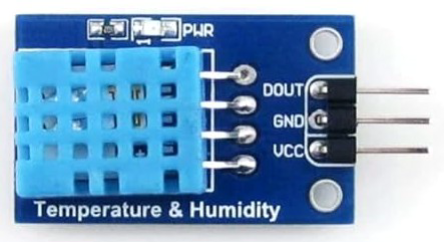
\includegraphics[width=0.53\textwidth]{Diagramas/temp.png}
\end{figure}

\subsection{Sensor de Luminosidad GY-30 (BH1750FVI)}

El GY-30 es un módulo que utiliza el circuito integrado BH1750FVI, un sensor de luz ambiental que convierte la iluminancia en una señal digital de 16 bits \cite{gy30}. La comunicación con el microcontrolador se realiza a través de la interfaz de bus I²C. Su respuesta espectral es similar a la del ojo humano, lo que lo hace ideal para aplicaciones de ajuste de brillo en pantallas \cite{gy30}.

Sus características destacadas son:


\begin{itemize}
    \item \textbf{Rango de medición:} 1 a 65,535 lux \cite{gy30}.
    \item \textbf{Tensión de alimentación (VCC):} 2.4 a 3.6V \cite{gy30}.
    \item \textbf{Interfaz:} Comunicación digital I²C, compatible con modo rápido (hasta 400 kHz) \cite{gy30}.
    \item \textbf{Tiempo de medición:} Típicamente 120 ms en el modo de alta resolución (H-Resolution Mode) \cite{gy30}.
\end{itemize}

\begin{figure}[H]
    \centering
    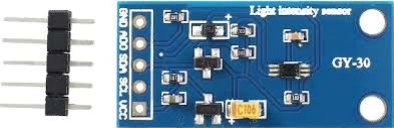
\includegraphics[width=0.6\textwidth]{Diagramas/lum.png}
\end{figure}
\subsection{Pantalla LCD Nextion NX4827P043-011R}

La Nextion NX4827P043-011R es una pantalla LCD-TFT de 4.3 pulgadas con funcionalidad táctil resistiva, diseñada para crear Interfaces Hombre-Máquina (HMI) \cite{nextion}. La comunicación con un microcontrolador se realiza mediante una interfaz serial TTL \cite{nextion}. Para el diseño de la interfaz gráfica se utiliza el software Nextion Editor \cite{nextion}.

Especificaciones técnicas:

\begin{itemize}
    \item \textbf{Resolución:} 480x272 píxeles \cite{nextion}.
    \item \textbf{Colores:} 65,536 colores (formato RGB 565) \cite{nextion}.
    \item \textbf{Alimentación recomendada:} 5V, 1.0A DC \cite{nextion}.
    \item \textbf{Memoria Flash:} 120 MB para almacenar fuentes e imágenes de la GUI \cite{nextion}.
\end{itemize}
